\documentclass[11pt]{article}
%ACENTOS
\usepackage[utf8]{inputenc}
\def\figurename{Fig.}
\def\tablename{Tabla}
\def\refname{Referencias}
\setlength{\parskip}{1em}

%PAQUETES
\usepackage{amsfonts,amsmath,amssymb}    % need for subequations
\usepackage{amsmath,latexsym}
\usepackage{graphics,color}
\usepackage{graphicx}
\usepackage{algpseudocode}
\usepackage[most]{tcolorbox}
\usepackage{hyperref} %Para colocar direcciones Web
\usepackage{booktabs} % Tablas
\usepackage[thinc]{esdiff} % Derivadas

%MARGEN
\setlength\topmargin{-0.5in}
\addtolength\oddsidemargin{-0.5in}
\setlength{\textheight}{23cm}
\setlength{\textwidth}{16cm}

%VARIABLES
\newcommand{\N}{\mathbb N}
\newcommand{\Z}{\mathbb Z}
\newcommand{\R}{\mathbb R}
\newcommand{\C}{\mathbb C}
\providecommand{\norm}[1]{\lVert#1\rVert}
%COLORES
\newcommand{\rojo}[1]{\textcolor[rgb]{1.00,0.00,0.00}{#1}}
\newcommand{\azul}[1]{\textcolor[rgb]{0.00,0.00,1.00}{#1}}
 
  
\begin{document}

\begin{center}
 \Large{\\ \\PROYECTO: Problema de iluminación} \\ \medskip
 \small{Elaborado por Diego Sánchez / Giselt Parra}\\ \medskip
 \footnotesize{16 de Marzo de 2020}
\end{center}

\begin{tcolorbox}[enhanced jigsaw,breakable,pad at break*=1mm, title= Puntos extremos de iluminación]

\vspace{0.25cm}
1) Generar una gráfica con tres curvas: la iluminación que genera cada bombilla sobre la
carretera y la curva de la iluminación total. Analice dicha gráfica e identifique aproximaciones para $x_{max}$, $x_{min}$ y $x_{eq}$, y denótelas por $x^0_{max}$, $x^0_{min}$ y $x^0_{eq}$, respectivamente.

\vspace{0.5cm}
2) Describir detalladamente una propuesta numérica, basada en el modelo de la sección
anterior, que involucre algún método numérico que le permita encontrar mejores aproximaciones a $x_{max}$, $x_{min}$ y $x_{eq}$. En caso de requerir aproximaciones iniciales de dichos
valores, use $x^0_{max}$, $x^0_{min}$ y $x^0_{eq}$
eq como iterados iniciales.

\vspace{0.5cm}
3) Programar la(s) rutina(s) derivada(s) de su propuesta numérica para obtener mejores aproximaciones a $x_{max}$, $x_{min}$ y $x_{eq}$.

\vspace{0.5cm}
4) Adicionalmente, usted deberá responder justificadamente las siguientes preguntas:

\vspace{0.25cm} \hspace{0.25cm}
4.1) ¿Qué distancia existe de $x_{min}$ a $x_{eq}$. Comente lo observado.

\vspace{0.25cm} \hspace{0.25cm}
4.2) ¿Los puntos de mayor iluminación se encuentran justo debajo de cada bombilla?

\vspace{0.25cm} \hspace{0.25cm}
4.3) ¿Qué ocurre con $x_{min}$ y $x_{eq}$ si p1 = p2 y h1 = h2?

\end{tcolorbox}
\noindent \textbf{Codigos}
\begin{tcolorbox}[colframe=blue!35!black, title=Códigos pregunta 3]
    Para toda la parte I: 
    aproximaciones\_precisas 
     \\
     Para el item 5.3:
    whatIf.py 
\end{tcolorbox}

\newpage
\vspace{0.5cm}
% === Poner aquí respuestas de la pregunta 1 ===
\textbf{Respuesta a la pregunta 1}

Las aproximaciones iniciales se determinan analizando la gráfica de $C(X)$ de forma aproximada, evaluando $n\in\N$ puntos discretos igualmente espaciados, denotemos a esos puntos como el conjunto $P=\{y_i=C(x_i) \mid x_i\in(0,30] , 0 \leq i \leq n \}$. Entonces  para aproximar $x_{max}$ se obtiene el mayor número en $P$, es decir, $max(P)=x^0_{max}$ análogamente para obtener una aproximación a $x_{min}$ se obtiene el menor número de $P$, esto es $min(P)=x^0_{min}$

Para $x_{eq}$  se hace un procedimiento similar para obtener una aproximación, utlizando también n puntos igualmente espaciados. Sea $L_a =  \{y_i=L_{1}(x_i) \mid x_i\in(0,30] , 0 \leq i \leq n \}$ y $L_b = \{y_i=L_{2}(x_i) \mid x_i\in(0,30] , 0 \leq i \leq n \}$. Luego haciendo la diferencia por cada elemento de $L_a$ con cada elemento de $L_b$ obtenemos $L_c$, finalmente $min(L_c) = x^0_{eq}$.

La función min y max encuentran el xi asociado a al yi mínimo y máximo respectivamente de P, así como de $L_c$

\begin{figure}[!h]
	
	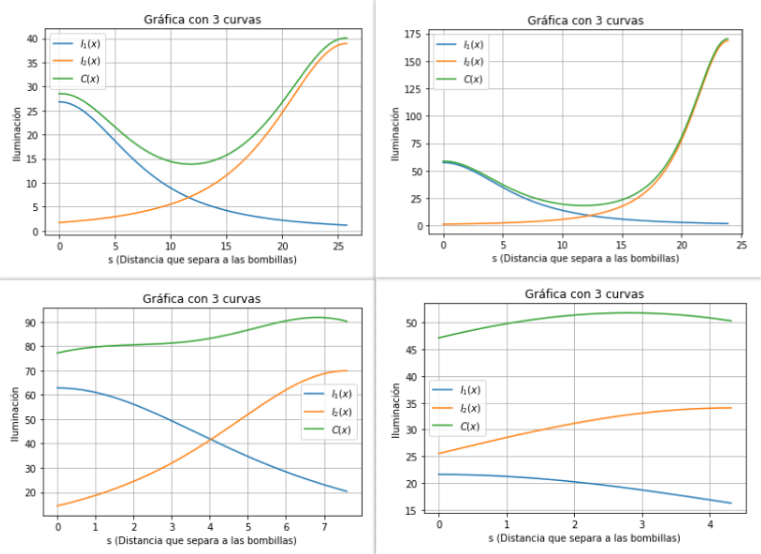
\includegraphics[keepaspectratio, width=15cm]{Imagenes/grafica.png}
	\caption{\\Fig. Gráfica de Iluminaciones \label{fig:grafica2}}
\end{figure}

\noindent \textbf{Respuesta a la pregunta 2}

Para obtener mejores aproximaciones para $x_{max}$, $x_{min}$ y $x_{eq}$ que las iniciales se, propone el siguiente método, teniendo como afirmación que $C(x)$ es continua $\forall x\in(0,30]$.

\begin{enumerate}
    \item Dado $x^0_{max}$, se calcula el punto en donde $\displaystyle \diff{C}{x} = 0$ alrededor de $x^0_{max}$ mediante el algoritmo de ceros de funciones bisección, en donde
    \begin{center}
        \begin{equation}
            \diff{C}{x} = \dfrac{3h_2p_2\left(s-x\right)}{\left(\left(s-x\right)^2+h_2^2\right)^\frac{5}{2}}-\dfrac{3h_1p_1x}{\left(x^2+h_1^2\right)^\frac{5}{2}}\label{eq:eq1}
        \end{equation}
    \end{center}
    \item Dado $x^0_{min}$ se calcula el punto en donde $\displaystyle \diff{C}{x} = 0$ alrededor de $x^0_{min}$ mediante el algoritmo de ceros de funciones bisección utilizando \eqref{eq:eq1}
    
    \item Dado $x^0_{eq}$, si existe, se calcula el punto en donde $\displaystyle L1(x)-L2(x) = 0$ alrededor de $x^0_{eq}$ mediante el algoritmo de ceros de funciones bisección. En donde:
    
    $$ L1(x)-L2(x) =  \dfrac{h_1p_1}{\left(x^2+h_1^2\right)^\frac{3}{2}}-\dfrac{h_2p_2}{\left(\left(s-x\right)^2+h_2^2\right)^\frac{3}{2}}$$
    
    Puede existir el caso en donde $L1(x)=L2(X)$, es decir, que las rectas no se intersecten, en este caso no se tendría el punto $x^0_{eq}$ y no se ejecutaría el paso 3
    
\end{enumerate}

\noindent \textbf{Respuesta a la pregunta 3}
\begin{tcolorbox}[colframe=blue!35!black, title=Códigos pregunta 3]
    aproximaciones\_precisas
\end{tcolorbox}

\noindent \textbf{Respuesta a la pregunta 4}
\begin{enumerate}
    \item La distancia  $|x_{eq} - x_{min}| \approx 0$ es aproximadamente 0 para la mayoría de los casos, excepto en los casos en donde $L_1(x)$ y $L_2(x)$ no se intersectan.


    \item Sí, en efecto, es lógico pensar eso ya que mientras más nos alejemos de una bombilla su intensidad luminosa disminuye, observándose que el comportamiento de $C(x)$ va decreciendo de izquierda a derecha, alcanza un mínimo, y después posiblemente dependiendo ya de los valores de p2 y h2 empiece a crecer. 
    
    \item Si $p1=p2$ y $h1=h2$ entonces las distancia $|x_{eq} - x_{min}|$ es 0 y vemos que el mínimo se alcanza alrededor de $s/2$ dado que las curvas $L1(x)$ y $L2(x)$ son espejos uno de las otras con respecto a el eje $y$.
    
    \begin{figure}[!h]
	    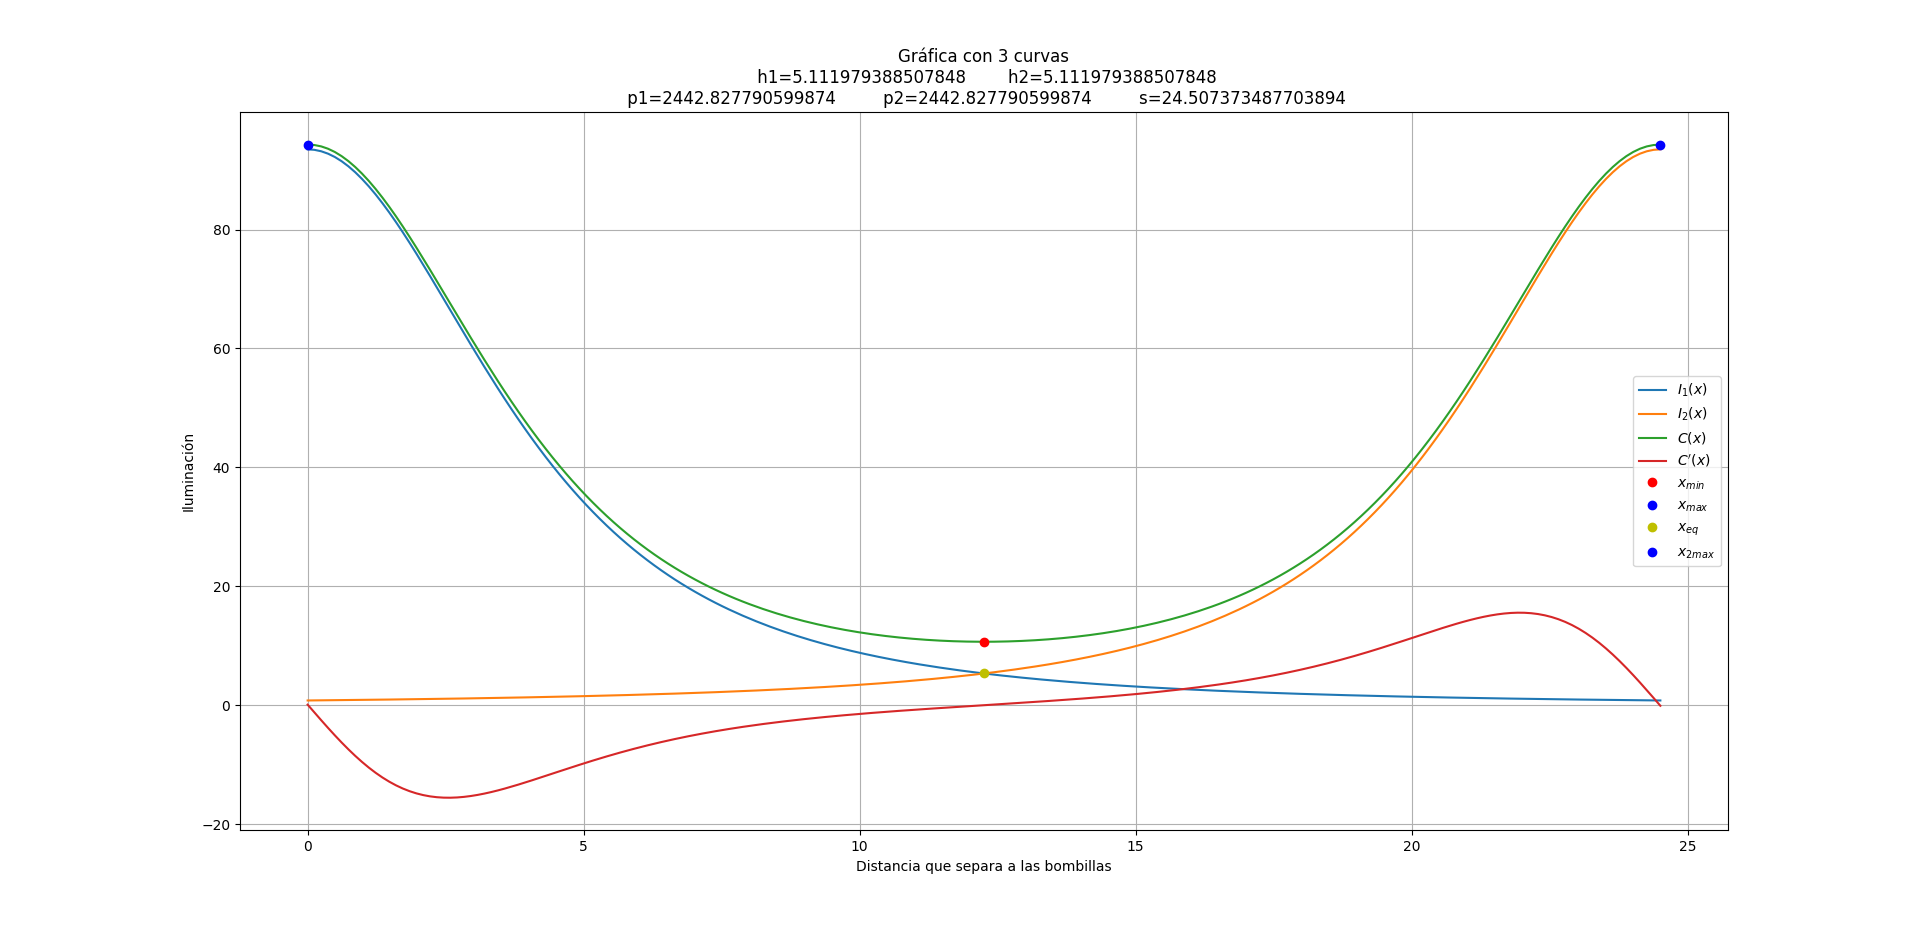
\includegraphics[keepaspectratio, width=15cm]{Imagenes/p1igualp2.png}
	    \caption{\\Fig. Fig. p1 = p2, h1 = h2 \label{fig:grafica2}}
	\end{figure}
    Para la imagen anterior considere el código p1igualp2.py y para las posteriores gráfica.py
    
    Como soporte, si reemplazamos en L1(x)-L2(x) los valores de p1 = p1 = p, h1 = h2 = h, mediante un despeje para hallar el valor de x tenemos que la solución está justo en la mitad del intervalo [0,s] siendo s/2 el punto x = xmin = xeq. Para ese cálculo se utilizó la herramienta WolframAlpha
    \begin{figure}[!h]
        	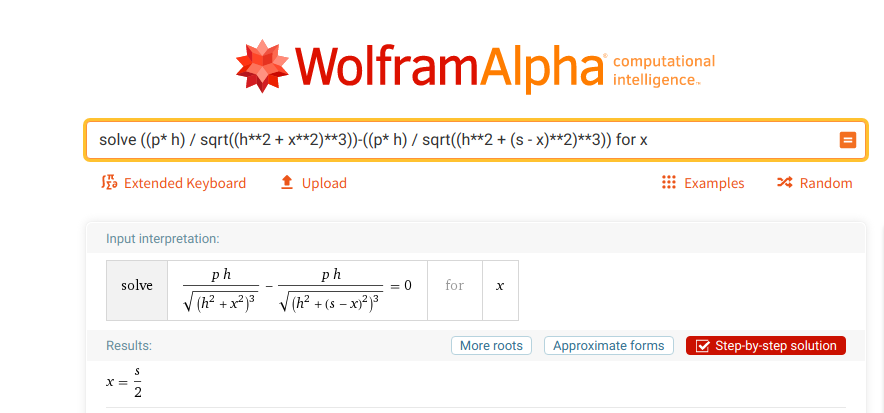
\includegraphics[keepaspectratio, width=15cm]{Imagenes/soporte.png}
        	\caption{\\Fig. Despeje de x cuando p1 = p2, h1 = h2 \label{fig:grafica3}}
    \end{figure}


\end{enumerate}

\begin{figure}[!h]
	
	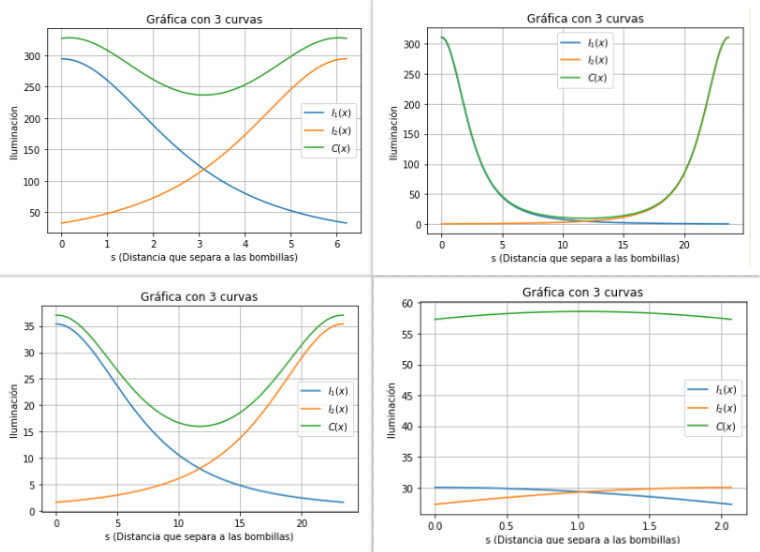
\includegraphics[keepaspectratio, width=15cm]{Imagenes/whatIf.png}
	\caption{\\Fig. p1 = p2, h1 = h2 \label{fig:grafica2}}
\end{figure}
\newpage
\vspace{0.5cm}
\begin{tcolorbox}[enhanced jigsaw,breakable,pad at break*=1mm, title= Pregunta 2]

\vspace{0.25cm}
1) Escribir una rutina que sea capaz de generar las gráficas de las Figuras 2, 3 y 4.

\vspace{0.5cm}
2) Responder justificadamente las siguientes preguntas:

\vspace{0.25cm} \hspace{0.25cm}
2.1) ¿El punto ($x_0, h^0_2$) es un punto mínimo, máximo o de silla?

\vspace{0.25cm} \hspace{0.25cm}
2.2) Observe que \nabla C(x, $h_2$) : $R^2$ $\to$  $R^2$ 
. Calcule, muy cuidadosamente el vector
\nabla C(x, $h_2$) y evalúelo en ($x_0, h^0_2$)
). Comente el resultado.

\vspace{0.25cm} \hspace{0.25cm}
2.3) Observe que \nabla^2 C(x, $h_2$) : $R^2$ $\to$ $R^{2x2}$
. Calcule, muy cuidadosamente a la matriz
\nabla^2 C(x, $h_2$) y evalúela en ($x_0, h^0_2$). Comente el resultado.

\vspace{0.25cm} \hspace{0.25cm}
2.4) ¿Los valores de \nabla C($x_0, h^0_2$) y \nabla^2 C($x_0, h^0_2$) están acorde con la respuesta dada en el ıtem 2.1)?

\vspace{0.5cm}
3) Describir detalladamente una propuesta numérica, basada en el modelo de la sección
anterior y las nuevas consideraciones sobre la variable h2, que involucre algún método
numérico que le permita encontrar mejores aproximaciones a ($x^*_{min}$, $h^*_2$).
\vspace{0.5cm}
4) Investigar sobre el Método $BFGS^2$
y describir su propósito. ¿Este método le resulta
de utilidad en su propuesta numérica?.



\vspace{0.5cm}
5) Programar y ejecutar BFGS usando C(x, $h_2$), ∇C(x, $h_2$), $x_0$ = ($x^0,h^0_2$). ¿Qué representa el valor $x_{k+1}$ retornado por BFGS en el contexto del problema de iluminación?

\end{tcolorbox}

\vspace{0.5cm}
\noindent \textbf{Respuesta a la pregunta 1}

\begin{tcolorbox}[colframe=blue!35!black, title=Códigos]
figuras3d.py
\end{tcolorbox}


\vspace{0.5cm}

    \noindent \textbf{Respuesta a la pregunta 2}
    \begin{enumerate}
        \item En todos los casos probados, el punto mejor iluminado entre los menos iluminados cuando x y $h_2$ varían, el punto ($x^0,h^0_2$) es un punto de silla.

            	
            \begin{figure}[!h]	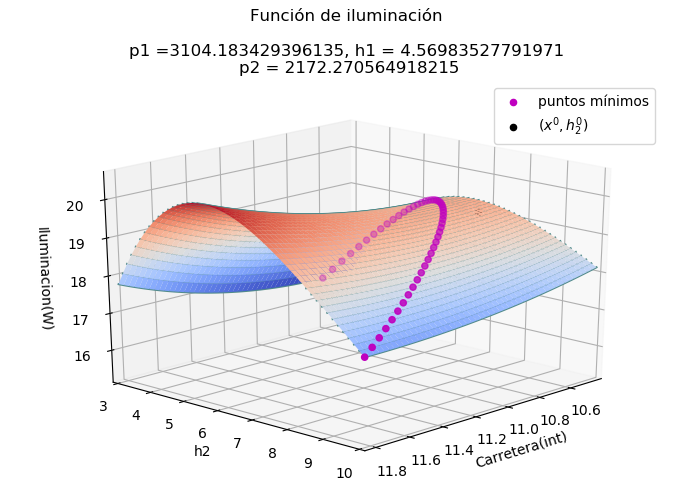
\includegraphics[keepaspectratio, width=15cm]{Imagenes/silla1.png}
            	\caption{\\Fig. Acercamiento de los peores puntos iluminados \label{fig:grafica3}}

            \end{figure}
            \begin{figure}[!h]
        	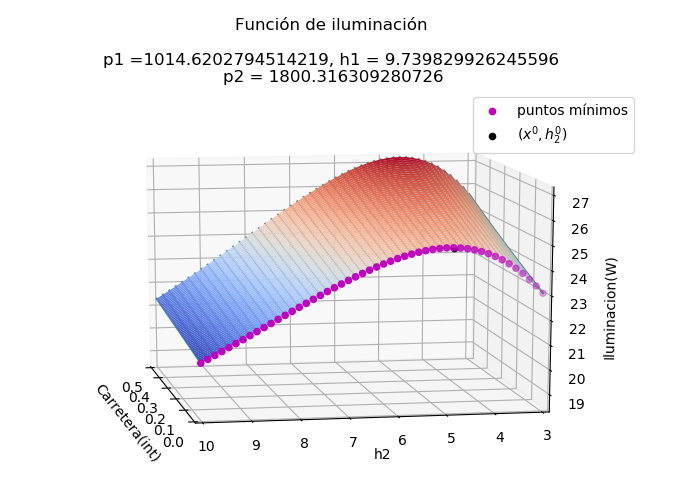
\includegraphics[keepaspectratio, width=15cm]{Imagenes/silla2.png}
            	\caption{\\Fig. Acercamiento de los peores puntos iluminados\label{fig:grafica3}}
            \end{figure}
    \item 
    \begin{tcolorbox}[colframe=blue!35!black, title=Códigos pregunta 3]
    punto\_inicial.py
\end{tcolorbox}
    Observacion: En los casos probados, cuando se evalua el vector gradiente en el punto de aproximación inicial, uno de los elementos del vector arroja un valor muy cercano a cero.

    \item
    \begin{tcolorbox}[colframe=blue!35!black, title=Códigos]
punto\_inicial.py
\end{tcolorbox}
    Observaciones: En la mayoria de los casos la mayoria de los elementos de la matriz Hessiana son negativos exceptuando $f_{xx}$ (el primer elemento de la primera columna y la primera fila). Esto tiene sentido dado que siguiendo el criterio de la matriz Hessiana, si el determinante de la matriz es negativo y este elemento es positivo, entonces el punto evaluado es un mínimo.
    \item
    Los valores calculados al evaluar el punto ($x^0,h^0_2$) a la rutina teniendo como resultados el vector gradiente y la matriz Hessiana sí están acordes con la respuesta dada en el item 1 dado a que se tomó en cuenta el criterio de la matriz Hessiana para la clasificación. Teniendo un punto critico que denominaremos como (x,y), éste se clasifica de la siguiente manera:
    
        \vspace{0.25cm}
        - Si el determinante es mayor que cero, entonces se procede a verificar si el elemento que corresponde a $f_{xx}$ en la matriz es positivo o negativo. Si es positivo entonces(x,y) es un mínimo. En el caso contrario, (x,y) es un máximo.
       
        \vspace{0.25cm}
        - Si el determinante es menor que cero entonces se concluye que la función tiene un punto silla en (x,y).
        
        \vspace{0.25cm}
        - Si el determinante es igual a cero el criterio no es concluyente, por lo tanto se debe buscar otra forma de determinar el comportamiento de la función. el ı́tem
        
        Algunos casos probados:
        
        \vspace{0.5cm}
        \begin{figure}[!h]
        	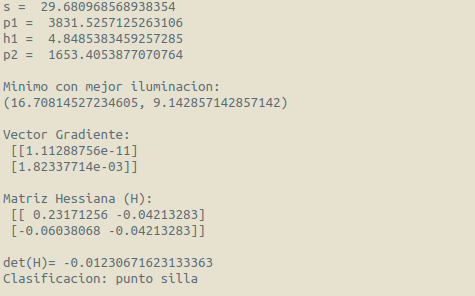
\includegraphics[keepaspectratio, width=10cm]{Imagenes/det1.png}
        	\caption{\\Fig. Los valores de \nabla C($x^0_0, h^0_2$) y \nabla^2 C($x^0_0, h^0_2$) \label{fig:grafica3}}
        \end{figure}
    
        \begin{figure}[!h]
        	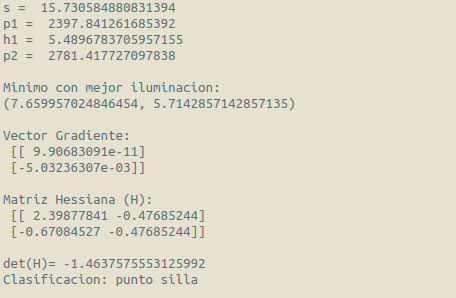
\includegraphics[keepaspectratio, width=10cm]{Imagenes/det2.png}
        	\caption{\\Fig. Los valores de \nabla C($x^0_0, h^0_2$) y \nabla^2 C($x^0_0, h^0_2$)\label{fig:grafica3}}
        \end{figure}

    \vspace{0.5cm}
    \noindent \textbf{Respuesta a la pregunta 3}
    \item 
        Para hallar la mejor aproximación ($x^*_0, h^*_2$) en un principio se planteó buscar los puntos críticos de C'(x,h2) a través de las raíces que podían ser obtenidos hallando el cero de dicha función.

        \begin{figure}[!h]
        	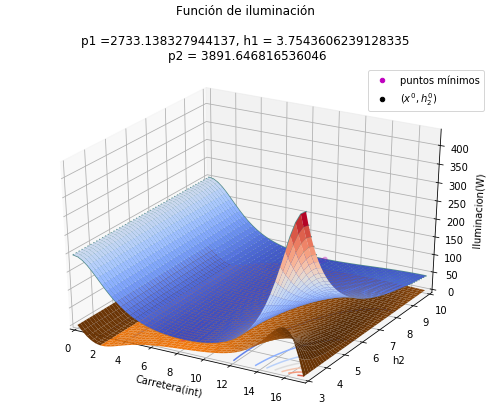
\includegraphics[keepaspectratio, width=13cm]{Imagenes/derivada3d.png}
        	\caption{\\Fig.  C(x,h2) y C’(x,h2) evaluado con h2 variante
        	\label{fig:grafica3}}
        \end{figure}
        \begin{figure}[!h]
        	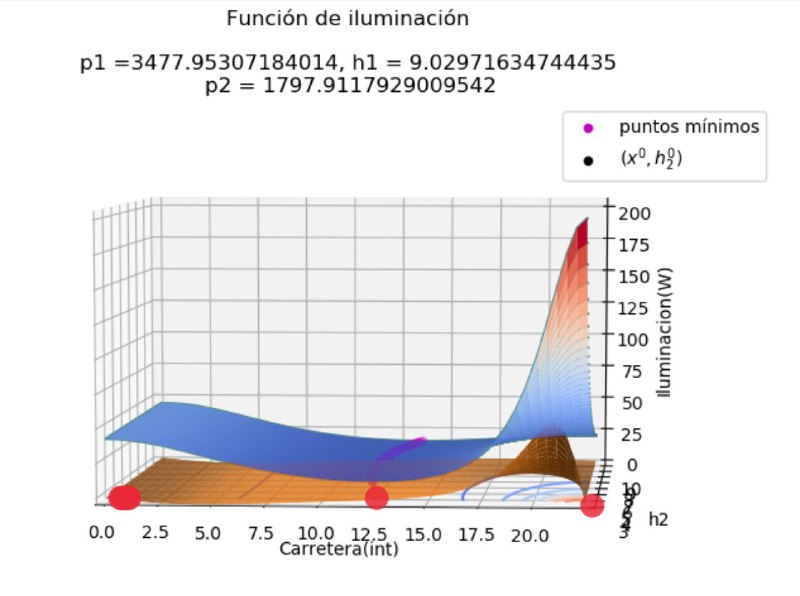
\includegraphics[keepaspectratio, width=15cm]{Imagenes/derivada3dp.jpeg}
        	\caption{\\Fig. Puntos críticos de C(x,$h_2$) evaluado con $h_2$ variante \label{fig:grafica3}}
        \end{figure}
        
        Sin embargo, de ésta forma se presenta el problema de clasificar dichos puntos críticos dado a que el punto mejor iluminado entre los menos iluminados puede resultar tanto un mínimo como un punto de silla, por tanto, determinar con certeza que el mayor entre estos mínimos y puntos de silla es el punto ($x^*,h^*_2$) no resulta viable. 
        
        La solución para obtener la mejor aproximación y determinar cuál de los puntos con peor iluminación es el mayor de todos se opta por hacer esta selección entre todos los puntos mínimos de la función por cada valor de $h_2$ mediante el método cero de función por bisección utilizada en la primera parte del proyecto dado a que hemos transformado un problema de tres dimensiones en la suma de un problema de dos. De esta manera, evitamos el problema de clasificación antes mencionado dado a que no se estudia sobre una figura de tres dimensiones donde puede darse el caso de obtener un punto silla.
        \begin{figure}[!h]
        	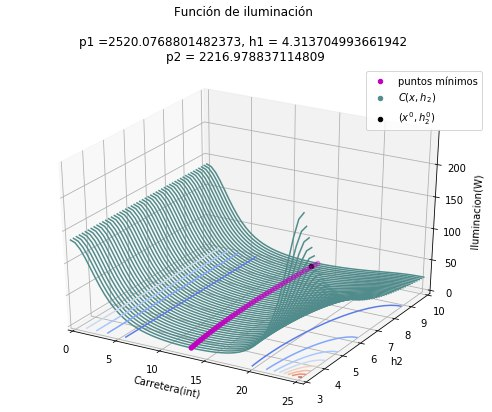
\includegraphics[h,keepaspectratio, width=13cm]{Imagenes/parte2.jpg}
        	\caption{\\Fig. C(x,$h_2$) evaluado con $h_2$ variante \label{fig:grafica3}}
        \end{figure}

        	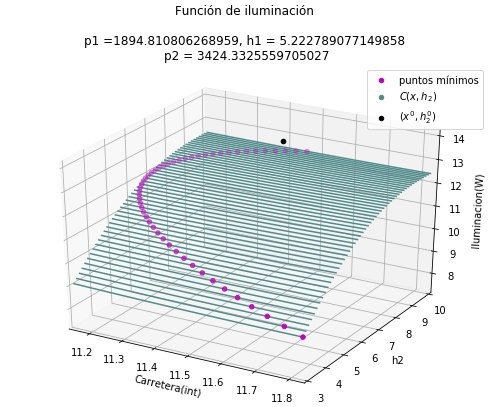
\includegraphics[keepaspectratio, width=13cm]{Imagenes/parte2_2.jpg}
        	\caption{\\Fig. C(x,$h_2$) evaluado con $h_2$ variante \label{fig:grafica4}}

        
        
    \vspace{0.5cm}
    \noindent \textbf{Respuesta a la pregunta 4}
    

    El método BFGS es un algoritmo de optimización utilizado para encontrar ceros de funciones o puntos críticos de una función, generalmente se utilizan si la matriz Jacobiana es costosa de calcular o no se tiene disponible.
    
    Una de las ventajas principales de BFGS es que la matriz Hessiana no necesita ser invertida si no que se aproxima por cada iteración.
    
    Dicho esto si resulta de utilidad aplicar aplicar BFGS a nuestra propuesta numérica.
    
    
    
    \vspace{0.5cm}
    \noindent \textbf{Respuesta a la pregunta 5}
    \begin{tcolorbox}[colframe=blue!35!black, title=Códigos]
BFGS.py
\end{tcolorbox}

    El vector $X_{k+1}$ representa el cero de la función $C'(x,h_2)$ es decir la mejor aproximación a $x*$ que determina el punto de mayor luminosidad entre los mínimos.

\end{enumerate}






%===============================================================================
% AQUI ESTA LA SECCCION DE LAS REFERENCIAS
\bibliographystyle{plain}
\bibliography{refs} %VEAN QUE AQUI SE COLOCA EL NOMBRE DEL ARCHIVO .BIB
\end{document}
